% This file was created with tikzplotlib v0.10.1.
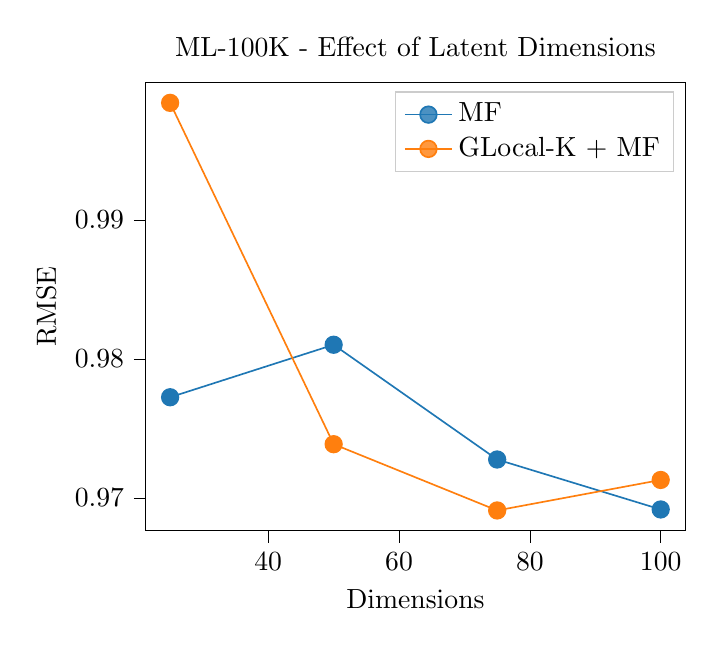
\begin{tikzpicture}

\definecolor{darkgray176}{RGB}{176,176,176}
\definecolor{darkorange25512714}{RGB}{255,127,14}
\definecolor{lightgray204}{RGB}{204,204,204}
\definecolor{steelblue31119180}{RGB}{31,119,180}

\begin{axis}[
legend cell align={left},
legend style={fill opacity=0.8, draw opacity=1, text opacity=1, draw=lightgray204},
tick align=outside,
tick pos=left,
title={ML-100K - Effect of Latent Dimensions},
x grid style={darkgray176},
xlabel={Dimensions},
xmin=21.25, xmax=103.75,
xtick style={color=black},
y grid style={darkgray176},
ylabel={RMSE},
ymin=0.96764244, ymax=0.99987376,
ytick style={color=black}
]
\addplot [semithick, steelblue31119180, mark=*, mark size=3, mark options={solid}]
table {%
25 0.977244616
50 0.981018901
75 0.972769618
100 0.96917814
};
\addlegendentry{MF}
\addplot [semithick, darkorange25512714, mark=*, mark size=3, mark options={solid}]
table {%
25 0.9984087
50 0.9738702
75 0.9691075
100 0.971299
};
\addlegendentry{GLocal-K + MF}
\end{axis}

\end{tikzpicture}
